\chapter{Introduction\label{ch:introduction}}

% \begin{enumerate}
% \item Welcome!

% \item Some Examples of Modeling

% \begin{enumerate}
%   \item WWI Fisheries data and the Volterra Principle; Scale Invasion
%   \item The SF Bay Model
%   \item Why do cities segregate (demos in NL instead of slides)
% \end{enumerate}

% \item These kinds of models were used for different purposes: to
%   support a decision (Bay Model) to explain a puzzling finding (LV) to
%   ask how possibly questions (Schelling)

% \item More complex models (Steve examples?)

% \item Who we are / who they are

% \item Overview of the course and objectives

% \item Pragmatics
%   \begin{enumerate}
%     \item room change?
%     \item laptops needed (can be borrowed from Van Pelt)
%     \item Book; course materials
%     \item Download Netlogo, will also need access to Excel
%     \item readings before class (other than today), assignments posted
%       to BB
%     \item group project at the end
%   \end{enumerate}

% \end{enumerate}

\section{What the Course Is About}

Welcome!
\vskip 12 pt
\noindent 

\subsection{Goals for the course}

\begin{enumerate}
\item Develop in the students  facility for engaging in model-based
  reasoning, whether in science or policy making or other
  applications.
\item Develop in the students facility for formulating models, whether in science or policy making or other
  applications.
\item Introduce students to model implementation.
\item Develop in the students facility for thinking critically about
  models, whether in science or policy making or other
  applications.
\end{enumerate}

\subsection{Objectives for the course (in service to the goals)}

\begin{enumerate}
\item Provide a general survey of models and modeling, whether in science or policy making or other
  applications.
\item Teach NetLogo as a modeling environment, especially for
  agent-based models.
\item Teach NetLogo programming, both for developing models in Net{-}Logo
  and for a gentle introduction to programming for modeling and
  analysis of models.
\item Support hands-on learning leading to design, implementation, and analysis
  of models in NetLogo.
\end{enumerate}

\subsection{Focal Topics}

\begin{enumerate}
\item Formulating models.

This comes with practice and is taught by examples and exercises.

\item Agent-based modeling.

We will focus for the most part on agent-based models. These, more than other types of models are perhaps the easiest for beginners to think about and create. They are a new and rapidly developing style of modeling, in which models are articulated in terms of interactions among individual agents. 

\item NetLogo.

NetLogo is a ``low floor, high ceiling'' development environment for agent-based modeling. It is inspired by the programming language Logo, which was originally created for the purpose of teaching children how to program. The NetLogo language remains easy for and accessible to beginners, and can be used for quite substantive modeling efforts. 

We will learn to program and develop models in NetLogo. The skills we acquire in doing so are largely transferable to other contexts.

\item Using models in deliberation.

Model formulation and model-based deliberation are the principal facets of ``thinking with models.'' Here we shall emphasize the principle of solution pluralism as a means for supporting model-based deliberation. As it happens, NetLogo has convenient facilities for this.

\end{enumerate}

\subsection{Structure of the course}

\begin{enumerate}
\item Will follow to a large extent the ``SAIL'' methods and
  philosophy: Structured, Active, In-class Learning.

Reading assignments should be done before class.
Most classes will be mostly given over to doing in-class exercises. These
are required. Some questions will be fairly easy and you should be
able to do them if you pay attention in the short lectures and
generally keep up with readings. Bs. Then there will be other
questions that you should be able to get if you prepare for class
(we'll have very definite material and instructions). As. During the
class exercises, we will be here and available to answer questions and
help you out. The spirit of the class sessions will be one of
collaboration for the sake of learning.

Grading: In-class exercises, plus the term project, and class
participation.
Maybe other assignments???

\item First $\approx$2/3 of course will focus on getting up to speed in
  NetLogo. Then we'll do more survey stuff as you, in parallel, plan
  and implement your term projects, your models.
\end{enumerate}

\noindent Go over syllabus.


\section{Modeling Examples}

% \begin{enumerate}
%   \item WWI Fisheries data and the Volterra Principle; Scale Invasion
%   \item The SF Bay Model
%   \item Why do cities segregate (demos in NL instead of slides)
% \end{enumerate}

\subsection{ WWI Fisheries data and the Volterra Principle; Scale
  Invasion}

 Read: \citet[chapters 1 and 2]{weisberg_2013}.

\subsection{San Franciso Bay model}

 Read: \citet[chapters 1 and 2]{weisberg_2013}.
See on Youtube:
\begin{itemize}
\item \url{https://www.youtube.com/watch?v=GjTA8Wxi1XA} (2:11 minutes,
  good)
\item \url{https://www.youtube.com/watch?v=zcetEPDEOFQ} (4:24 minutes,
  good)
\item ``Model Saves SF Bay from Ecological Disaster '' from {\it
    Wired}. Good background info, 3:51. \url{https://www.youtube.com/watch?v=MiL_TvY1a9g}
\end{itemize}

\subsection{Segregation}

Schelling model, in NetLogo; see Models Library, Sample Models, Social Science.

\subsection{Traffic Basic}

In NetLogo; see Models Library, Sample Models, Social Science.

\subsection{Castello Ursino Catania}



See ``Agent-Based Simulation of Pedestrian Behaviour in Closed Spaces:
A Museum Case Study ,'' by Alessandro Pluchino, Cesare Garofalo,
Giuseppe Inturri, Andrea Rapisarda and Matteo Ignaccolo (2014),
\url{http://jasss.soc.surrey.ac.uk/17/1/16.html},
\citep{pluchino2014}.

See Figures \ref{fig:CastelloUrsinoCatania_1} and
\ref{fig:CastelloUrsinoCatania_2}, following. Their NetLogo model is
[will be]
posted on Canvas.

\newpage

\begin{figure}[htbp] %  figure placement: here, top, bottom, or page
   \centering
   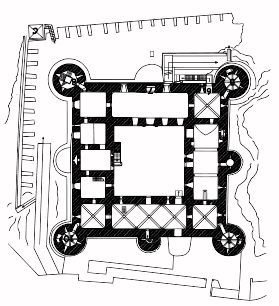
\includegraphics[width=\textwidth]{figures/Fig01.png}  
   \caption{Castello Ursino Catania: The castle, now museum, ground floor plan.} % using random-seed 22478
   \label{fig:CastelloUrsinoCatania_1}
\end{figure}

\begin{figure}[htbp] %  figure placement: here, top, bottom, or page
   \centering
  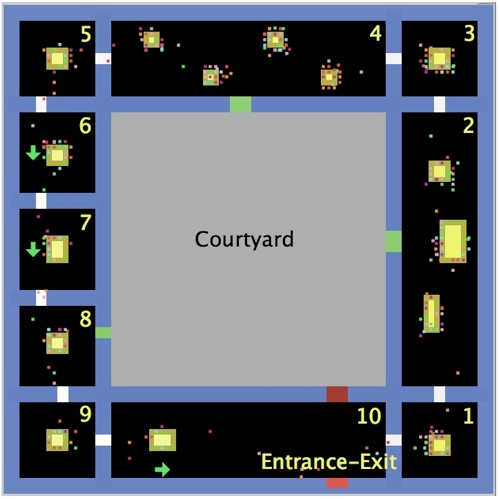
\includegraphics[width=\textwidth]{figures/Fig02.png}  
   \caption{Castello Ursino Catania: The NetLogo model user interface.} % using random-seed 22478
   \label{fig:CastelloUrsinoCatania_2}
\end{figure}

\subsection{Knapsack}

Example of a \emph{constrained optimization model} (COModel).

\clearpage\newpage

\section{Thinking about Models: Some Basic Distinctions}


Note that these models are apt for, can be used for, different
purposes, e.g.,  to
  support a decision (Bay Model), to explain a puzzling finding (LV), to
  ask ``How possibly?'' questions (Schelling).

Some distinctions:
\begin{enumerate}
\item ``Three Kinds of Models'' \citep[chapter 2]{weisberg_2013}:
  concrete models (e.g., SF Bay model), mathematical models (e.g.,
  Lotka-Volterra model, knapsack model), and computational models
  (e.g., Segregation, Traffic Basic).

Focus of the course is on computational models and specifically on
agent-based models (ABMs, aka: individual-based models or IBMs).
But much of what we will learn will apply to other kinds of models.

\item Parametric versus strategic decisions (and models).

Parametric: decision maker (agent) makes a choice, Nature acts, possibly
randomly, and the decision maker is rewarded (positively or
negatively). Example: San Francisco Bay model, knapsack model.

Strategic: decision maker (agent) makes a choice, Nature acts, possibly
randomly, and the decision maker is rewarded (positively or
negatively), depending in part on decisions made by other
agents/decision makers. Lotka-Volterra. Segregation. Traffic Basic. Castello Ursino Catania.

In this course we'll look at both kinds of decisions and models of them.

\item Insight versus decision models.

Decision: San Francisco Bay model, knapsack models, and (to a degree) Lotka-Volterra.

Insight (but not decision): Segregation, Traffic Basic. 


But: Lotka-Volterra, and Castello Ursino Catania.

\item Descriptive versus exploratory models.

A distinction developed by Steven Bankes and others. See \citep{bankes_1993,bankes_lempert_popper_2002} for starters.

\end{enumerate}

\section{Agent-Based Modeling}

\citep{bankes_lempert_popper_2002,epstein_axtell_1996,gilbert_2008,grimm_railsback_2005,miller_page_2007,railsback_gramm_netlogo_2012,wilensky_rand_2015}


\section{Solution Pluralism: Key to Thinking with Models}

our present project, employs in an essential way the perspective of what we call \emph{solution pluralism} \citep{sok_etal_gecco_2012,sscr_redistricting_2013}.
It will be helpful for framing our project to describe briefly this conceptual point of departure. So, a word about that now.

Solution pluralism in the context of modeling is the principle of
obtaining multiple solutions for a model and using the resulting
\emph{corpus} of solutions to inform deliberation and decision making.
The principle appears elsewhere as well, notably in observation and
mesurement, where it is standard practice to obtain a sample of
(often, ideally independent) observations or measurements, and then to reason
from the sample. This is pervasive and required in most cases; it is
what we doing in making survey samples and in weighing small
quantities multiple times.  


In the context of modeling, the principle of solution pluralism is
often realized in sensitivity anlysis, where multiple solutions of a
model type are obtained by varying one or more parameters in an
instance of the model type. Similarly, when constrained optimization
is involved it is standard to obtain multiple solutions to a model for
the sake of estimating the Pareto frontier of the decision space, as
one or more parameters vary.  Corpora of solutions to model instances
are also standardly obtained when the models have stochastic elements,
as in Monte Carlo and discrete event simulations.

% our present project, employs in an essential way the perspective of what we call \emph{solution pluralism} \citep{sok_etal_gecco_2012,sscr_redistricting_2013}.
% It will be helpful for framing our project to describe briefly this conceptual point of departure. So, a word about that now.

% Solution pluralism in the context of modeling is the principle of
% obtaining multiple solutions for a model and using the resulting
% \emph{corpus} of solutions to inform deliberation and decision making.
% The principle appears elsewhere as well, notably in observation and
% mesurement, where it is standard practice to obtain a sample of
% (often, ideally independent) observations or measurements, and then to reason
% from the sample. This is pervasive and required in most cases; it is what we doing in making survey samples and in weighing small quantities multiple times.  

% In the context of modeling, the principle of solution pluralism is often realized in sensitivity anlysis, where multiple solutions of a model type are obtained by varying one or more parameters in an instance of the model type. Similarly, when constrained optimization is involved it is standard to obtain multiple solutions to a model for the sake of estimating the Pareto frontier of the decision space, as one or more parameters vary.
% Corpora of solutions to model instances are also standardly obtained
% when the models have stochastic elements, as in Monte Carlo and
% discrete event simulations.


\section{NetLogo}

Ten minute overview.

\section{For Next Time}

\begin{enumerate}
\item Install NetLogo on your computer.
\item Bring your computer to class.
\item See the syllabus and do the assigned readings. In particular,
  read \citep[chapter 2, pages 45--68]{wilensky_rand_2015} and read in the {\it NetLogo User Manual}
  (\url{http://ccl.northwestern.edu/netlogo/docs/} and installed on
  your computer
  with the NetLogo distribution):
\begin{itemize}
\item Tutorial \#1: Models
\item Tutorial \#2: Commands
\item Tutorial \#3: Procedures
\end{itemize}
Also, we'll be reading these, so you may as well get started:
\begin{itemize}
\item Interface Guide
\item Info Tab Guide
\item Programming Guide
\end{itemize}
See Figure \ref{fig:NetLogoUserManual}.

\begin{figure}[htbp] %  figure placement: here, top, bottom, or page
   \centering
   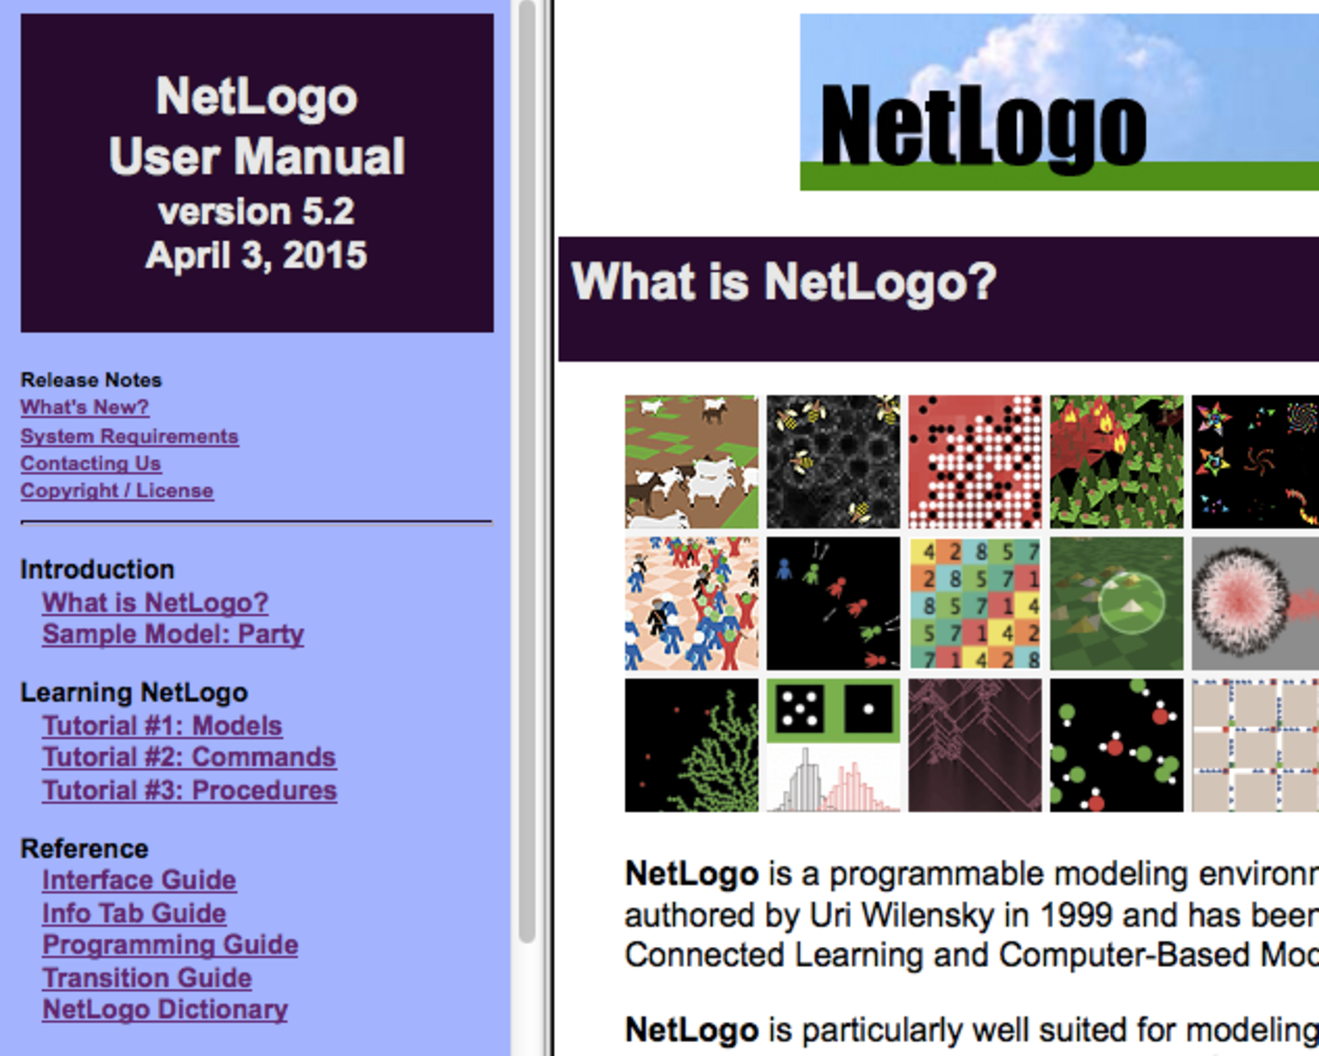
\includegraphics[width=\textwidth]{figures/NetLogoUserManual.pdf}  
   \caption{NetLogo User Manual.} 
   \label{fig:NetLogoUserManual}
\end{figure}
\end{enumerate}

\newpage\clearpage

\section{For More Information}

On agent-based modeling: \citep{bankes_lempert_popper_2002,epstein_axtell_1996,gilbert_2008,grimm_railsback_2005,miller_page_2007,railsback_gramm_netlogo_2012,wilensky_rand_2015}

\vfill
\noindent\verb+$Id: introduction.tex 4950 2015-09-13 18:31:27Z sok $+